\documentclass{article}
\usepackage[utf8]{inputenc} 
\usepackage[T1]{fontenc}    
\usepackage{graphicx}       
\usepackage{hyperref}       
\usepackage{amsmath} 
\usepackage{authblk}
\usepackage{tocloft}

\newcommand{\MyDocTitle}{Distributed Quantum Computing workflows with ColonyOS}

\title{\MyDocTitle}

\hypersetup{
    colorlinks=true,
    linkcolor=blue,
    urlcolor=blue,
    citecolor=green,
    pdftitle={\MyDocTitle},
    pdfauthor={Karim Elgammal, Erik Källman, Thor Wikfeldt},
}

\makeatletter
\renewenvironment{abstract}{
  \if@twocolumn
    \section*{\abstractname}
  \else
    \begin{center}
      {\bfseries \abstractname\vspace{-.5em}\vspace{\z@}}
    \end{center}
    \quotation
  \fi}
  {\if@twocolumn\else\endquotation\fi}
\makeatother

\setcounter{tocdepth}{1}

\setlength{\cftbeforesecskip}{0.5ex}

\begin{document}
\author[1,2]{Karim Elgammal}
\author[2]{Erik Källman}
\author[1,2]{Thor Wikfeldt}
\affil[1]{\href{https://enccs.se/}{ENCCS - EuroCC National Competence Center Sweden}}
\affil[2]{\href{https://www.ri.se/en}{RISE - Research Institute of Sweden}}
\date{April 2025}

\maketitle

\begin{abstract}
Quantum computing is evolving rapidly across the globe, and Europe is no exception, with significant investments powering new research frontiers. However, a key challenge lies in efficiently orchestrating complex computations that often require integrating classical high performance computing (HPC) resources with diverse quantum hardware. Here is an overview on \href{https://colonyos.io/}{ColonyOS}, an open source meta-operating system designed to address this need by orchestrating distributed computing workflows across heterogeneous environments (including cloud, HPC, standalone workstations, and can be extended towards quantum systems). This report discusses the benefits of such orchestration, highlight key ColonyOS features, and showcase example applications in managing quantum computations. ColonyOS has the potential to streamline hybrid calculations and accelerate the path towards quantum accelerated supercomputing.
\end{abstract}

\tableofcontents

\section{Introduction}\label{sec:introduction}
Quantum computing is evolving rapidly across the globe, and Europe is no exception, with significant investments powering new research frontiers. However, a key challenge lies in efficiently orchestrating complex computations that often require integrating classical high-performance computing (HPC) resources with diverse quantum hardware. Here is an overview on \href{https://colonyos.io/}{ColonyOS}, an open-source meta-operating system designed to address this need by orchestrating distributed computing workflows across heterogeneous environments (including cloud, HPC, standalone workstations, and can be extended towards quantum systems). This report discuss the benefits of such orchestration, highlight key ColonyOS features, and showcase example applications in managing quantum computations. ColonyOS has the potential to streamline hybrid calculations and accelerate the path towards quantum-accelerated supercomputing.

\section{The need for distributed quantum computing}\label{sec:need-distributed-quantum}

Quantum computing scientists and engineers across different disciplines need to leverage classical and quantum resources in their workflows. They need to develop and test algorithms locally on their personal computers before scaling them up to more complex environments. This iterative process involves expanding the algorithm in terms of parameters, noise models, system complexity, and other details. The next step is to run the workflow on a quantum computer with a few qubits. Of course, due to the limited accessibility to quantum hardware or the limited qubits available, a common target of that workflow is to run it on a powerful computer, which can be an HPC resource capable of simulating hundreds of qubits with the help of some packages and software development kits. Such solutions have the potential to use extensive resources, making it suitable to distribute the workflow over multiple compute resources. For reusability, users require the ability to access those resources seamlessly, saving time by storing profiles of the hardware that this specific workflow can run on across different European compute infrastructures.

\section{Leveraging ColonyOS for distributed quantum computing}\label{sec:leveraging-colonyos}

\href{https://colonyos.io/}{ColonyOS} is an open-source meta-operating system designed to streamline workload execution across diverse and distributed computing environments, including cloud, edge, HPC, and IoT. More details are provided in the \href{https://ar5iv.labs.arxiv.org/html/2403.16486}{arXiv} article. This capability makes it well-suited for managing complex, resource-intensive quantum computing tasks. The software is available under the MIT Licence and can be accessed via \href{https://github.com/colonyos}{GitHub}. Comprehensive \href{https://github.com/colonyos/tutorials}{tutorial notebooks} are also available to facilitate onboarding.

\section{Key features of ColonyOS for quantum-accelerated supercomputing}\label{sec:key-features}

ColonyOS offers several key features that could enable managing the quantum computing workflows and advancing quantum-accelerated supercomputing.

\subsection{Distributed microservice architectures}\label{subsec:microservices}

ColonyOS employs a microservices architecture, where independent executors handle specific tasks. This design supports distributed quantum computing by allowing quantum tasks to be executed across geographically dispersed quantum and classical computing resources in a hybrid fashion. Executors can be deployed independently and scaled horizontally, ensuring efficient parallel processing.

\subsection{Workflow orchestration}\label{subsec:orchestration}

The platform enables users to define complex, multi-step workflows across distributed executors. This is particularly beneficial for quantum computing applications, which often require iterative execution of quantum circuits, optimisation steps (e.g., variational quantum eigensolver (VQE) algorithms), and hybrid quantum-classical computations. ColonyOS manages dependencies and execution sequencing, ensuring seamless operation across diverse computational systems.

\subsection{Scalability}\label{subsec:scalability}

Given the potential for node failures in distributed infrastructures, ColonyOS is designed to reassign tasks dynamically if an executor fails. This approach minimises computation disruptions and enhances overall system reliability.

\subsection{Platform-Agnostic integration}\label{subsec:integration}

ColonyOS can operate across multiple platforms, including cloud services and HPC environments. This flexibility aligns with the hybrid quantum-classical infrastructures often required for quantum computing workflows, allowing for efficient orchestration of tasks on both classical supercomputers and quantum processors.

The distributed architecture, task orchestration capabilities, and scalability of ColonyOS make it a powerful solution for managing quantum computing workflows. By leveraging ColonyOS, users can efficiently coordinate tasks across quantum and classical computing environments, accelerating the development and deployment of quantum algorithms that are advancing toward further use in quantum-accelerated supercomputing.

\section{Example: orchestrating and visualising quantum computing workflows with ColonyOS}\label{sec:example}

The following snippets are related to an example where ColonyOS orchestrated Qiskit variational calculations with different noise models. ColonyOS generated multiple simulations accounting for different noise models. For more implementation details and related code, please visit the blog post \href{https://www.ekprojectjournal.com/doku.php?id=projects:quantum:distributed}{here}.

ColonyOS serialises Qiskit objects, metrics, and metadata from each part of the workflow into an SQLite database. This database is then exposed to localhost via a simple Flask API, which connects to a React frontend that presents two key views of the results data. Both views display the same data and allow ranking across a set of metrics but do so in different ways:
\begin{itemize}
    \item The first way is through the metrics table---a simple (in-development) table that displays each noise simulation computation along with data from its related variational simulation, as shown in Figure~\ref{fig:metrics_table}.
    \item The second way is through a workflow graph showing how each step in the workflow is connected and which steps depend on its information, as shown in Figure~\ref{fig:graph_unfiltered}.
\end{itemize}

\begin{figure}[htbp]
    \centering
    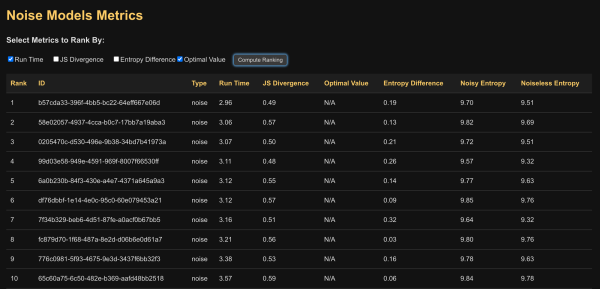
\includegraphics[width=1.0\linewidth]{img/metrics_table.png}
    \caption{The ColonyOS metrics table displaying results from variational simulations with different noise models.}
    \label{fig:metrics_table}
\end{figure}

\begin{figure}[htbp]
    \centering
    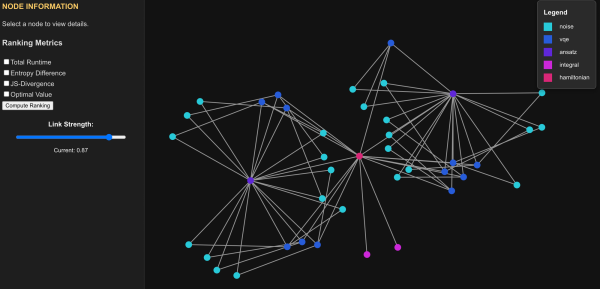
\includegraphics[width=1.0\linewidth]{img/graph_unfiltered.png}
    \caption{The ColonyOS workflow graph visualising the connections between different computation steps.}
    \label{fig:graph_unfiltered}
\end{figure}

In Figure~\ref{fig:graph_unfiltered}, the legend explains which part of the calculation workflow the nodes correspond to. A node information panel displays metrics of the selected node. It allows to compute rankings across nodes (similar to the metrics table shown in Figure~\ref{fig:metrics_table}) while rescaling and labelling nodes as a function of rank, as depicted in Figure~\ref{fig:graph_filtered}. Workth-mentioning that with more complex systems and calculations, the database could present a denser graph providing easily searchable sets of data.

\begin{figure}[htbp]
    \centering
    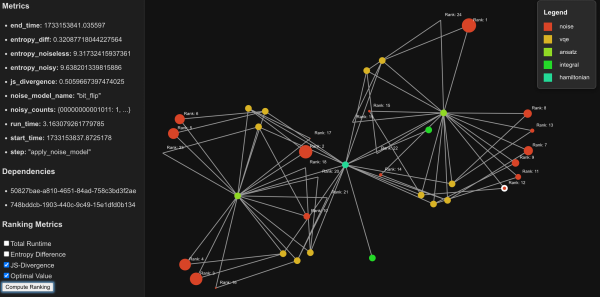
\includegraphics[width=1.0\linewidth]{img/graph_filtered.png}
    \caption{The workflow graph ranked based on specific metrics, highlighting performance differences.}
    \label{fig:graph_filtered}
\end{figure}

\section{Conclusion}\label{sec:conclusion}
These examples highlight ongoing efforts to integrate \href{https://colonyos.io/}{ColonyOS} into quantum computing workflows---a promising step toward distributed computing orchestration. This work also leveraged graph data analytics to view and analyse
quantum computation outcomes. \href{https://colonyos.io/}{ColonyOS}, as part of \href{https://eucloudedgeiot.eu/decentralised-edge-to-cloud computing-with-colonyos-recording-now-available/}{the European Compute Continuum Initiative}, could become a vital part at the
orchestration layer for the \href{https://eurohpc-ju.europa.eu/index_en}{EuroHPC-JU} hybrid quantum-classical infrastructure, enabling seamless utilisation of resources like \href{https://eurohpc-ju.europa.eu/advancing-european-quantum-computing-signature-procurement contract-eurohpc-quantum-computer-located-2024-09-26_en}{LUMI-Q} and \href{https://eurohpc-ju.europa.eu/signature-procurement-contract eurohpc-quantum-computer-located-spain-2025-01-28_en}{MareNostrum Q} with the existing HPC classical resources. To explore ColonyOS further, check out the \href{https://github.com/colonyos}{GitHub repository} and the \href{https://github.com/colonyos/tutorials}{available tutorials}.

\section{Acknowledgement}\label{sec:acknowledgement}

This report is based on work by \href{https://www.ri.se/sv/person/erik-kallman}{Erik Källman}, first presented at the \href{https://enccs.github.io/qas2024/_downloads/e7a4c465a0e6318304e776636c9d317f/QAS-COS.pdf}{Nordic
Quantum Autumn School 2024} and further elaborated in an accompanying blog post \href{https://www.ekprojectjournal.com/doku.php id=projects:quantum:distributed}{here}. The original content can be found in \href{https://www.ekprojectjournal.com/doku.php?id=projects:quantum:distributed}{Erik Källman's blog}. The concepts and implementations have been adapted and expanded with permission to showcase the potential of \href{https://colonyos.io/}{ColonyOS} in distributed quantum computing workflows. We thank \href{https://www.ri.se/sv/person/erik-kallman}{Erik Källman} for his work in this area and for sharing his insights during the \href{https://enccs.github.io/qas2024/cos/}{Nordic Quantum Autumn School 2024}.
\end{document}
